% Author biographies retained from main_book_v04.tex.
    \extrachap{About the Authors}

    \addcontentsline{toc}{chapter}{About the Authors}

\begin{authorbiography}[{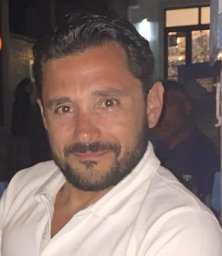
\includegraphics[width=\linewidth,height=1.25in,clip,keepaspectratio]{figures/kdeliparaschos.jpg}}]{Kyriakos M. Deliparaschos} (Senior Member, IEEE) received his B.Eng. (Hons) in Electronic Engineering and M.Sc. in Mechatronics from De Montfort University, UK, and the National Technical University of Athens (NTUA), Greece. He earned his Ph.D. from the Department of Signals, Control and Robotics, School of Electrical and Computer Engineering, NTUA, Greece. He currently holds a Special Teaching Staff position in the Department of Electrical Engineering, and Computer Science and Engineering (EECSE) at the Cyprus University of Technology (CUT), Cyprus. He has held academic and research positions at New York College and IST College in Athens, Greece; NTUA, Greece; CUT, Cyprus; Trinity College Dublin, Ireland; and Cranfield University, UK. His research interests include embedded systems, reconfigurable hardware acceleration, sensor fusion, resilient cyber-physical systems, intelligent control, real-time robotic navigation, and medical robotics for minimally invasive surgery.
\end{authorbiography}


\begin{authorbiography}[{
\includegraphics[width=\linewidth,height=1.25in,clip,keepaspectratio]{figures/goliva.jpg}}]{Gabriele Oliva} (Senior Member, IEEE) received the M.Sc and the Ph.D. degrees in computer science and automation engineering from the University Roma Tre of Rome, Italy, in 2008 and 2012, respectively. He is currently an Associate Professor in automatic control with the University Campus Bio-Medico of Rome, Italy, where he directs the Complex Systems \& Security Laboratory (CoserityLab). Since 2022, he is an Associate Editor for the IEEE Control Systems Letters Journal. Moreover, he has been an Associate Editor for the Conference Editorial Board of the IEEE Control Systems Society and for PLOS ONE. His main research interests include distributed multi-agent systems, optimisation, decision-making, maritime situation awareness, and critical infrastructure protection.
\end{authorbiography}

\begin{authorbiography}[{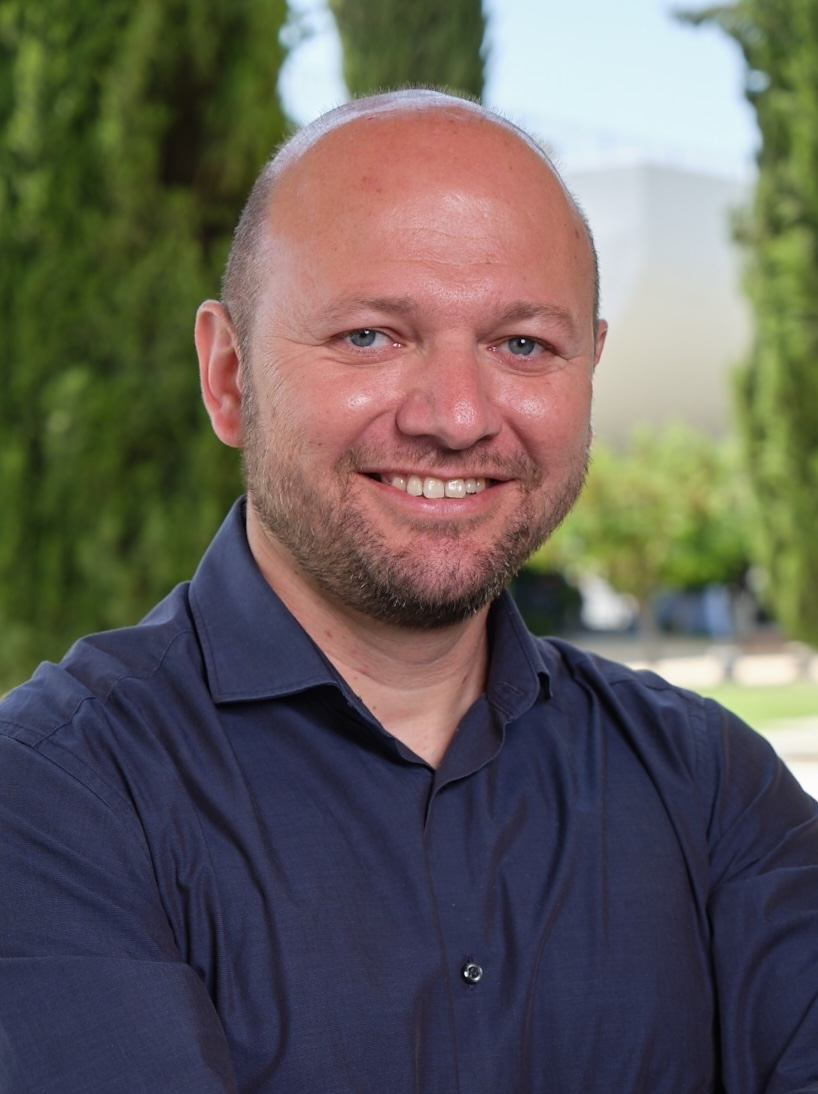
\includegraphics[width=\linewidth,height=1.25in,clip,keepaspectratio]{figures/themis4-papers.jpg}}]{Themistoklis Charalambous}~(Senior Member, IEEE) received the BA (First Class
Honours) and M.Eng. (Distinction) degrees in Electrical and Information Sciences from Trinity College, University of Cambridge, and the Ph.D. degree from the Control Laboratory, Department of Engineering, University of Cambridge.
%
Following his PhD, he held research and teaching positions at
Imperial College London, the University of Cyprus, KTH Royal Institute of Technology, and Chalmers University of Technology.
%
In 2017, he joined the Department of Electrical Engineering and Automation, School of Electrical Engineering, Aalto University, as an Assistant Professor; he was awarded the
title of Academy Research Fellow by the Academy of Finland in 2018 and was promoted to Associate Professor in 2020.
%
In September 2021, he joined the Department of Electrical and Computer Engineering, University of Cyprus, as a tenure-track Assistant Professor.
In May 2022, he received an ERC Consolidator Grant for the project ``MINERVA: Emerging Cooperative Autonomous Systems: Information for Control and Estimation.''
Since May 2026, he has been a tenured Associate Professor at the University of Cyprus. He is also a Visiting Professor at Aalto University and, since April 2023, at the FinEst Centre for Smart Cities.
%In September 2021, he continued his academic career at the University of Cyprus, where he joined the Department of Electrical and Computer Engineering as a tenure-track Assistant Professor. In May 2022, he was awarded an European Research Council (ERC) Consolidator Grant for the research project “MINERVA: Emerging Cooperative Autonomous Systems: Information for Control and Estimation.” From May 2026, he was appointed as a tenured Associate Professor at the University of Cyprus. He also remains affiliated with Aalto University as a Visiting Professor and, since April 2023, serves as a Visiting Professor at the FinEst Centre for Smart Cities.
%
%Prof. Charalambous is an Associate Editor of \textsc{IEEE Transactions on Automatic Control}
\end{authorbiography}

